\documentclass[11pt, a4paper, titlepage]{article}
\setlength{\parindent}{0pt}

%%%%%%%% paquetes %%%%%%%%
%\usepackage[lmargin=2cm,rmargin=2cm,top=1.5cm,bottom=2cm]{geometry}
\usepackage[T1]{fontenc}
\usepackage[utf8]{inputenc}
\usepackage[spanish,es-tabla]{babel}
\usepackage{amsmath}
\usepackage{amssymb,amsfonts,latexsym,cancel}
\usepackage{fancyhdr}
\usepackage{titlesec}
\usepackage{titling}
\usepackage{anyfontsize}
\usepackage{color}
\usepackage[dvipsnames]{xcolor}

\usepackage{csquotes}   
\usepackage[style=numeric-comp, sorting=none, block=par]{biblatex} 
\DeclareFieldFormat{title}{\bfseries\emph{#1}}
\definecolor{softblack}{RGB}{74, 71, 71} 
\DeclareFieldFormat{howpublished}{\textcolor{softblack}{\mdseries{#1}}}
\DeclareFieldFormat{labelnumberwidth}{\mkbibbold{#1\adddot}}
\setlength\bibitemsep{2.5\itemsep}
\renewcommand*{\newunitpunct}{\addspace}
\renewcommand*{\finentrypunct}{\addspace}
\usepackage{listings}
\usepackage{graphicx}
\usepackage[colorlinks = true,
			linkcolor = black,
			urlcolor = black,
			citecolor = blue ]{hyperref}

%%%%%%%% encabezado y pie de página %%%%%%%%
%\pagestyle{fancy}
%\fancyhead{}
%\fancyfoot{}
%\fancyfoot[R]{\thepage}
%\fancyfoot[L]{2º Trabajo Optimización Heurística}
%\renewcommand{\headrulewidth}{0pt}

%%%%%%%% formato de títulos y subtítulos %%%%%%%%

\definecolor{gray75}{gray}{0.75}
\newcommand{\hsp}{\hspace{20pt}}
\titleformat{\section}[hang]{\huge\bfseries}{\thesection\hsp\textcolor{gray75}{|}\hsp}{0pt}{\huge\bfseries}
\titlespacing{\section}{0pt}{0pt}{15pt}
\titleformat{\subsection}[hang]{\Large\bfseries}{\thesubsection\hsp}{0pt}{\Large\bfseries}
\titlespacing{\subsection}{0pt}{35pt}{15pt}
\titleformat{\subsubsection}[hang]{\large\bfseries}{\thesubsubsection\hspace{10pt}}{0pt}{\large\bfseries} 
\titlespacing{\subsubsection}{0pt}{20pt}{0pt}

%\titleformat{\section}[block]{\LARGE\bfseries}{\thesection.}{1mm}{}
%\titlespacing{\section}{0pc}{5.5ex}{1pc}
%\titleformat{\subsection}[block]{\Large\bfseries}{\thesubsection.}{1mm}{}
%\titlespacing{\subsection}{1.5pc}{5.5ex}{1pc}



\begin{document}

	\begin{titlepage}
    	\begin{center}
        	\hrulefill

        	\vspace{0.5cm}
        	{\bf\fontsize{25}{0}{\selectfont{Optimización Heurística\\[0.5cm]}}}
        	\fontsize{15}{0}{\selectfont{Evaluación de EAs\\[0.5cm]}}
        	\hrulefill
        	\vspace{6.0cm}
    	\end{center}

    	\centering
    	{\Large Daniel Tomás Sánchez\\ Aarón Cabero Blanco \\ Pablo Bautista 				Frías \par}
    	\vspace{2cm}
    	{\Large 03/01/2020 \par}
	\end{titlepage}

\newpage

%\renewcommand{\contentsname}{\fontsize{22}{0}{\selectfont{Índice}}}
%{\Large \tableofcontents}

\tableofcontents

\newpage

\section{Introducción}
En esta prática, el objetivo es la comparación y evaluación de diferentes algoritmos evolutivos (EAs). Para ello, además de evaluarlos, se deberá previamente  implementar un nuevo algoritmo evolutivo, el cual se explicará a continuación.
\section{Descripción del los algoritmos evolutivos}
Por un lado, se nos pidió implementar nosotros a mano un nuevo algoritmo evolutivo. Respecto al algoritmo de la práctica anterior, el actual sigue siendo un DE (Differential Evolution) pero, en este caso, se nos pidió cambiar dos operadores: el operador de cruce y el operador de mutación. En este caso, el operador de cruce es binomial, frente al exponencial de la práctica 1, y el operador de mutación es de/best/1 frente al de/rand/1 de la anterior. Este algoritmo parece ser mejor que el de la práctica anterior ya que, a la hora de realizar la mutación, se emplea el mejor genoma de la población por lo que, a primera vista, parece que convergerá más rápido.

\vspace{5mm}

Por otro lado, a la hora de elegir un algoritmo de una biblioteca que nosotros quisiéramos, nos decantamos por el SADE debido a una gran fama en su eficiencia que, como veremos después, hemos podido comprobar nosotros mismos.

\section{Distribución del código}
El código contiene toda la parte del algoritmo implementado por nosotros y un programa principal que es el que ejecutará las funciones de esta práctica. Este programa principal, denominado $benchmarking.py$ es el encargado de realizar la funcionalidad pedida y que, tras ejecutarla, crea diferentes archivos:

\begin{itemize}
\item \textbf{benchmarking.out}: contiene los resultados de nuestro algoritmo y del SADE, en las secciones $BASIC\_DE$ y $SADE$ respectivamente, los valores estadísticos (media, mediana, min, max y desv\_est) de los dos anteriores, los resultados del test de kruskal y los fitness medios de cada función.
\item \textbf{tableDE.png}: es la tabla que contiene los valores estadísticos nombrados anteriormente para cada función cuando se usa optimiza mediante nuestro DE.
\item \textbf{tableSADE.png}: es la tabla que contiene los valores estadísticos nombrados anteriormente para cada función cuando se usa optimiza mediante nuestro SADE.
\item \textbf{tableWhitney.png}: es la tabla que contiene el test de Wilcoxon comparando ambos algoritmos.
\end{itemize}
Además, se generan diferentes diagramas de caja comparando los dos algoritmos juntos por cada función.

\section{Output de la ejecución}
En este apartado vamos a ver cuáles son las diferentes salidas que tiene nuestro código. Para ello, veremos las diferentes tablas que se generar junto con una breve descripcion explicando cada una de ellas. Además, veremos solo algún diagrama de caja para, como dijimos antes, compara los algoritmos en cada función.
\subsection{Valores estadísticos}
Aquí veremos las tablas con los valores estadísticos tanto para nuestro algoritmo como para el SADE.
\subsubsection{Valores estadísticos DE}
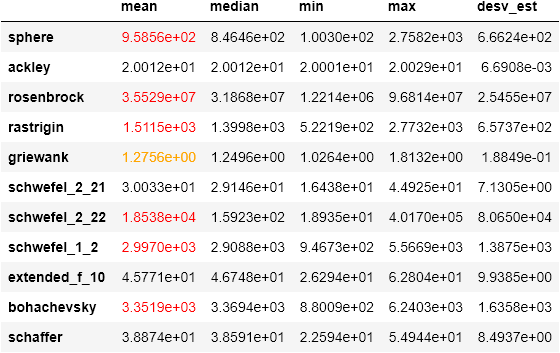
\includegraphics[width=\textwidth]{tableDE.png}
Descripción de la imagen.
\subsubsection{Valores estadísticos SADE}
\begin{center}
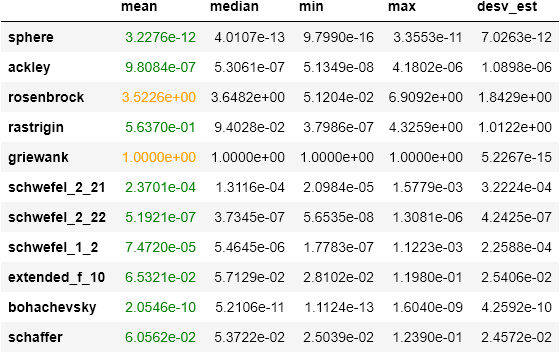
\includegraphics[width=\textwidth]{tableSADE.png}
\end{center}
Descripción de la imagen.
\subsection{Evaluación de EAs}
Cabe destacar que en cuanto a la evaluación de EAs, únicamente se va a realizar el test de Kruskal y el de Wilcoxon, pero no el de Friedman ya que para él es necesario un tercer algoritmo con el que comparar, cosa que no tenemos.
\begin{center}
\includegraphics[scale=0.85]{tableWhitney.png}
\end{center}
Descripción de la imagen.
\subsection{Diagramas de caja (boxplots)}
\begin{center}
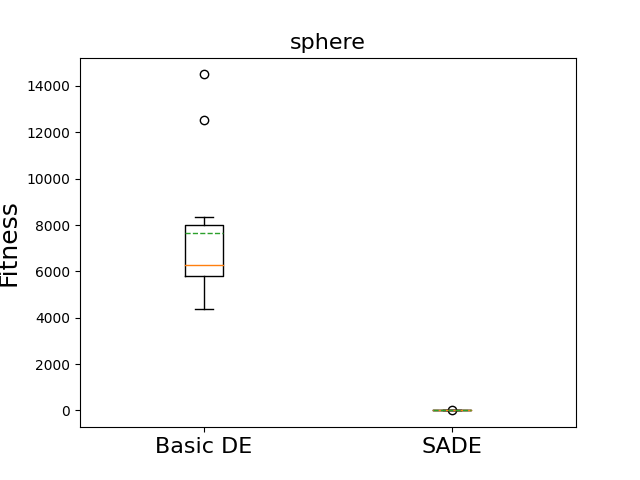
\includegraphics[scale=0.85]{sphere}
\end{center}
Descripción de la imagen.
\begin{center}
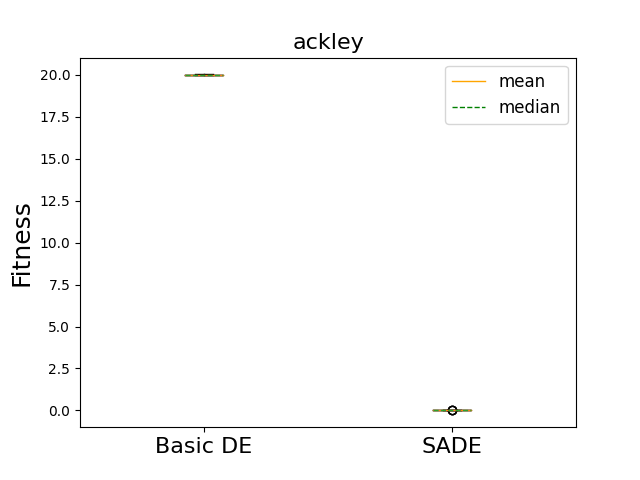
\includegraphics[scale=0.85]{ackley}
\end{center}
Descripción de la imagen.
\begin{center}
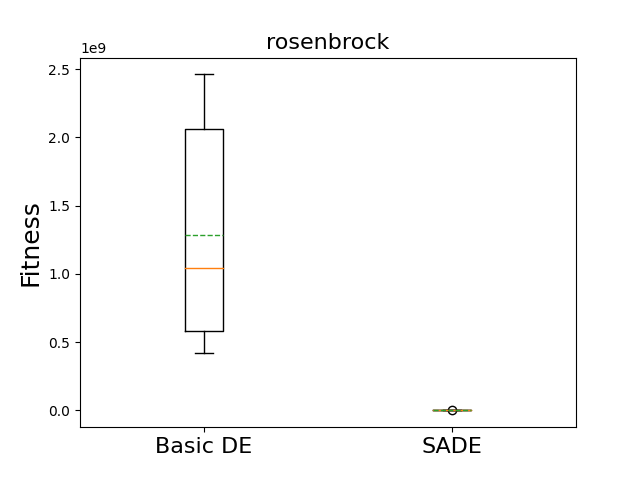
\includegraphics[scale=0.85]{rosenbrock}
\end{center}
Descripción de la imagen.
\begin{center}
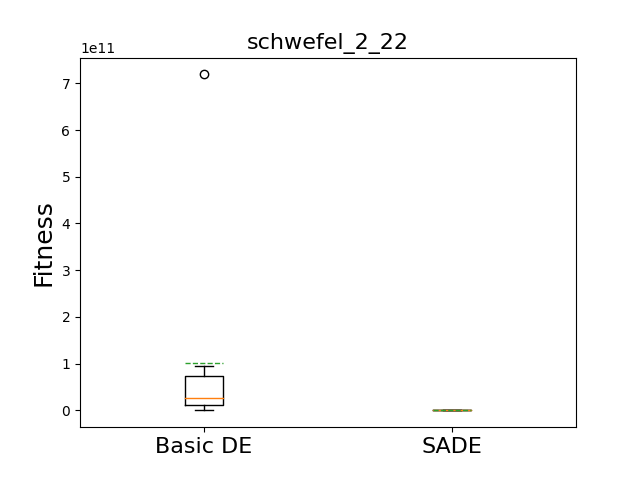
\includegraphics[scale=0.85]{schwefel_2_22}
\end{center}
Descripción de la imagen.
\section{Conclusión}
Pues aquí se pone algo de peloteo y a tomar por culo.
\end{document}
